% Options for packages loaded elsewhere
\PassOptionsToPackage{unicode}{hyperref}
\PassOptionsToPackage{hyphens}{url}
%
\documentclass[
  12pt,
]{article}
\title{Air Quality in Ukraine post Ukraine-Russia Dispute}
\usepackage{etoolbox}
\makeatletter
\providecommand{\subtitle}[1]{% add subtitle to \maketitle
  \apptocmd{\@title}{\par {\large #1 \par}}{}{}
}
\makeatother
\subtitle{\url{https://github.com/rachel-gordon823/FontanieGordonWeinberg_ENV872_EDA_FinalProject}}
\author{Shirley Fontanié, Rachel Gordon, and Julia Weinberg}
\date{}

\usepackage{amsmath,amssymb}
\usepackage{lmodern}
\usepackage{iftex}
\ifPDFTeX
  \usepackage[T1]{fontenc}
  \usepackage[utf8]{inputenc}
  \usepackage{textcomp} % provide euro and other symbols
\else % if luatex or xetex
  \usepackage{unicode-math}
  \defaultfontfeatures{Scale=MatchLowercase}
  \defaultfontfeatures[\rmfamily]{Ligatures=TeX,Scale=1}
  \setmainfont[]{Times New Roman}
\fi
% Use upquote if available, for straight quotes in verbatim environments
\IfFileExists{upquote.sty}{\usepackage{upquote}}{}
\IfFileExists{microtype.sty}{% use microtype if available
  \usepackage[]{microtype}
  \UseMicrotypeSet[protrusion]{basicmath} % disable protrusion for tt fonts
}{}
\makeatletter
\@ifundefined{KOMAClassName}{% if non-KOMA class
  \IfFileExists{parskip.sty}{%
    \usepackage{parskip}
  }{% else
    \setlength{\parindent}{0pt}
    \setlength{\parskip}{6pt plus 2pt minus 1pt}}
}{% if KOMA class
  \KOMAoptions{parskip=half}}
\makeatother
\usepackage{xcolor}
\IfFileExists{xurl.sty}{\usepackage{xurl}}{} % add URL line breaks if available
\IfFileExists{bookmark.sty}{\usepackage{bookmark}}{\usepackage{hyperref}}
\hypersetup{
  pdftitle={Air Quality in Ukraine post Ukraine-Russia Dispute},
  pdfauthor={Shirley Fontanié, Rachel Gordon, and Julia Weinberg},
  hidelinks,
  pdfcreator={LaTeX via pandoc}}
\urlstyle{same} % disable monospaced font for URLs
\usepackage[margin=2.54cm]{geometry}
\usepackage{longtable,booktabs,array}
\usepackage{calc} % for calculating minipage widths
% Correct order of tables after \paragraph or \subparagraph
\usepackage{etoolbox}
\makeatletter
\patchcmd\longtable{\par}{\if@noskipsec\mbox{}\fi\par}{}{}
\makeatother
% Allow footnotes in longtable head/foot
\IfFileExists{footnotehyper.sty}{\usepackage{footnotehyper}}{\usepackage{footnote}}
\makesavenoteenv{longtable}
\usepackage{graphicx}
\makeatletter
\def\maxwidth{\ifdim\Gin@nat@width>\linewidth\linewidth\else\Gin@nat@width\fi}
\def\maxheight{\ifdim\Gin@nat@height>\textheight\textheight\else\Gin@nat@height\fi}
\makeatother
% Scale images if necessary, so that they will not overflow the page
% margins by default, and it is still possible to overwrite the defaults
% using explicit options in \includegraphics[width, height, ...]{}
\setkeys{Gin}{width=\maxwidth,height=\maxheight,keepaspectratio}
% Set default figure placement to htbp
\makeatletter
\def\fps@figure{htbp}
\makeatother
\setlength{\emergencystretch}{3em} % prevent overfull lines
\providecommand{\tightlist}{%
  \setlength{\itemsep}{0pt}\setlength{\parskip}{0pt}}
\setcounter{secnumdepth}{5}
\ifLuaTeX
  \usepackage{selnolig}  % disable illegal ligatures
\fi

\begin{document}
\maketitle

\newpage
\tableofcontents
\newpage
\listoftables 
\newpage 
\listoffigures 
\newpage

\hypertarget{rationale-and-research-questions}{%
\section{Rationale and Research
Questions}\label{rationale-and-research-questions}}

\begin{quote}
During periods of war and geopolitical conflicts, environmental
pollution and degraded air quality is a common effect experienced by
nations subject to violent attacks. Specifically, the use of explosive
weapons can cause extensive damage to urban buildings and
infrastructure, resulting in hazardous dust, debris, and other air
particles that can have lasting health impacts on affected populations
(Dathan 2020).
\end{quote}

\begin{quote}
On February 24, 2022 Russia invaded Ukraine due to geopolitical
conflicts between the two nations. Russia's invasion has consisted of
multiple missile attacks throughout Ukraine, causing extensive damage to
urban infrastructure, reducing buildings to rubble and creating
dangerous explosions that have enormous potential to raise air pollution
levels. Therefore, in this project, we examine two different Ukrainian
cities that have experienced attacks since Russia's invasion and explore
air quality levels of these cities both before and during the war.
\end{quote}

\begin{quote}
As the conflict has been ongoing throughout all of March 2022, we chose
to analyze air quality data from March 2022 and 2021. We chose to
include data from the same month in 2021 to be able to compare air
quality levels during the war to the levels before to control for
weather and temperature variations that occur throughout different
months. Additionally, we were interested in exploring air quality levels
of two cities that are in different geographic locations and have
experienced at least one missile attack by Russia during March 2022. For
air quality indicators, we wanted to look at both PM 2.5 and PM 10, as
the levels of these particulate matters increase from sources such as
construction sites and fires and can have lasting effects on human
health (EPA, Particulate Matter Basics). PM2.5 are very fine inhalable
particles that are 2.5 micrometers or smaller, whereas PM10 are less
than 10.5 micrometers (EPA, Particulate Matter Basics). Lastly, we
wanted to look at two cities that differed in economic profiles
industrial manufacturing activity, as industrial manufacturing
activities can affect air quality levels (Parrett 2020).
\end{quote}

\begin{quote}
Based on these criteria, we chose to explore air quality levels of Lviv,
Ukraine and Dnipro, Ukraine. Lviv, a western-Ukranian city known as the
country's cultural capital, has experienced various missile attacks
since the initial Russian invasion (Anna 2022). Dnipro is a primarily
industrial, eastern-Ukranian city that has also been attacked at least
once during the Russian invasion (Lister et al.~2022). As these cities
differ in both geographical locations and industrial activity, they were
chosen as our cities to compare.
\end{quote}

\begin{quote}
The data analyzed was retrieved from the Air Quality Historical Data
Platform created by the World Air Quality Indices as this data source
had sufficient raw data for PM2.5 and PM10 levels across both March 2021
and March 2022 for both Lviv and Dnipro. From this dataset, we explored
the following research questions:
\end{quote}

\begin{quote}
\begin{enumerate}
\def\labelenumi{\arabic{enumi})}
\tightlist
\item
  Are there significant differences in air quality levels between
  affected Ukrainian cities during the Russian invasion?
\item
  Are there significant differences in air quality levels in affected
  Ukrainian cities before and during the Russian attacks?
\end{enumerate}
\end{quote}

\newpage

\hypertarget{dataset-information}{%
\section{Dataset Information}\label{dataset-information}}

\begin{quote}
Data for this project was retrieved from the World Air Quality Indices'
Air Quality Historical Data Platform (The World Air Quality Project).
The World Air Quality Index is a non-profit started in 2007 that is
working to increase transparency for air quality data in order to
improve pollution awareness. The World Air Quality Index created the Air
Quality Historical Data Platform in 2014 in order to provide information
on how location-based air quality is changing over time.
\end{quote}

\begin{quote}
Data in this report looks at PM10 and PM2.5 air pollution. The World Air
Quality Index provides ranges for air quality health and the numbers are
differentiated for PM2.5 and PM10. Table 1 provides the ranges for good,
moderate, poor, and unhealthy air quality levels. Historical data sets
available through the World Air Quality Index span a 36-month time
frame, and data used in this report is from 2019-2022. The data was
collected for two cities Dnipro and Lviv, located in Eastern and Western
Ukraine respectively. The air-quality monitoring station in Lviv is
called Steeldrum and the air-quality monitoring station in Dnipro is
called Vulytsya-Pavla Nirinberha, 4-6.
\end{quote}

\begin{quote}
Initially once accessing our first csv dataset (outlined in Table 1), we
processed the UkraineData by omitting missing values (the NA's) from the
PM2.5 and PM 10 values. Then, we set the ``numeric'' class of the date
column to a ``date'' class. Then, we wrangled the processed version of
the Ukraine data and created four subsets by city, month, and year. Each
city, Dnipro and Lviv, is being evaluated for air quality during the
month of March and in years 2021 and 2022.
\end{quote}

\begin{quote}
Now we have four new data sets; Dnipro 2021, Dnipro 2022, Lviv 2021, and
Lviv 2022, all showing PM2.5 and PM10 values for days in March. We then
binded the rows for both Dnipro 2021 and Dnipro 2022, called
FULL\_DNIPRO. We also binded rows for Lviv 2021 and Lviv 2022, called
FULL\_LVIV.
\end{quote}

\begin{quote}
In our exploratory analysis, we wanted to look at mean, maximum,
minimum, and the standard deviation for PM2.5 and PM10 values in Dnipro
and Ukraine. We used the group\_by function to group by City, and the
summarize function to include mean, maximum, minimum, and standard
deviation of the PM values. Additionally, within the exploratory
analysis we binded FULL\_Dnipro and FULL\_LVIV in order to create a dot
plot showing the air quality ranges our data demonstrated. We then
plotted this data with ggplot using scale\_fill\_gradient2 to color-code
data by health-hazard level. Furthermore, we wanted to look at PM2.5 and
PM10 values comparing Dnipro and Lviv in solely March 2022 -- during the
time of the missile attacks. To do this analysis, we wrangled the Dnipro
2022 and Lviv 2022 to create a dataset with both cities, that includes
both PM values, for solely March 2022. The important difference is that
we are not looking at 2021 values in this dataset. Table 2 outlines all
of our working data sets and what they each contain.
\end{quote}

\newpage

\textbf{Table 1}

\begin{longtable}[]{@{}lll@{}}
\toprule
Data File Name & Column Name & Data Type \\
\midrule
\endhead
UkraineData & City & Factor (Dnipro and Lviv) \\
UkraineData & Date & Factor (later converted to date object) \\
UkraineData & pm25 & Integer (PM2.5 values) \\
UkraineData & pm10 & Integer (PM10 values) \\
\bottomrule
\end{longtable}

\textbf{Table 2}

\begin{longtable}[]{@{}ll@{}}
\toprule
Data File Name & Description \\
\midrule
\endhead
UkraineData & (Raw) Ukraine air quality data \\
Ukraine\_Processed & (Processed) Ukraine air quality data, w/o na's \\
Dnipro\_2021 & Dnipro PM2.5 + PM10, Mar 2021 \\
Dnipro\_2022 & Dnipro PM2.5+ PM10, Mar 2022 \\
Lviv\_2021 & Lviv PM 2.5 + PM10, Mar 2021 \\
Lviv\_2022 & Lviv PM 2.5 + PM10, Mar 2022 \\
FULL\_LVIV & Lviv\_2021 + Lviv\_2022 combined \\
FULL\_Dnipro & Dnipro\_2021 + Dnipro\_2022 combined \\
FULL\_Air\_quality & Dnipro\_2022 + Lviv\_2022 combined \\
Full-air\_quality\_21\_22 & FULL\_LVIV + FULL\_Dnipro combined \\
\bottomrule
\end{longtable}

\newpage

\hypertarget{exploratory-analysis}{%
\section{Exploratory Analysis}\label{exploratory-analysis}}

\begin{quote}
To begin our exploratory analysis of the air quality data, we created
dot plots to map out what range of our quality our data fell into
(Figures 1 \& 2). The data is color coded with green denoting good air
quality conditions, yellow is moderate conditions, and red is showing
air quality that is poor and likely hazardous to health. Attached is a
table showing a breakdown for air quality metrics (Table 3). This dot
plot was created to show the range in which our data falls in terms of
air quality health. Additionally, we determined the summary statistics
of the PM2.5 and PM10 (Tables 4 + 5).
\end{quote}

\textbf{Table 3}

\begin{longtable}[]{@{}lll@{}}
\toprule
AQI Category & PM2.5 & PM10 \\
\midrule
\endhead
Good & 0 to 15.5 & 0 to 54 \\
Moderate & 15.5 to 35.5 & 54 to 150 \\
Poor & 35.5 to 150 & 150 to 250 \\
Unhealthy & 150+ & 250+ \\
\bottomrule
\end{longtable}

\newpage

\begin{figure}
\centering
\includegraphics{Fontanie_Gordon_Weinberg_Project_files/figure-latex/plot of PM25 air pollution by cityyear-1.pdf}
\caption{PM2.5 Air Pollution Distribution}
\end{figure}

\hfill\break

\begin{longtable}[]{@{}lrrrr@{}}
\caption{PM2.5 Levels by City}\tabularnewline
\toprule
City & Mean & Min & Max & Std Dev \\
\midrule
\endfirsthead
\toprule
City & Mean & Min & Max & Std Dev \\
\midrule
\endhead
Dnipro & 49.41546 & 4 & 160 & 25.91608 \\
Lviv & 60.51086 & 8 & 518 & 34.79405 \\
\bottomrule
\end{longtable}

\newpage

\begin{figure}
\centering
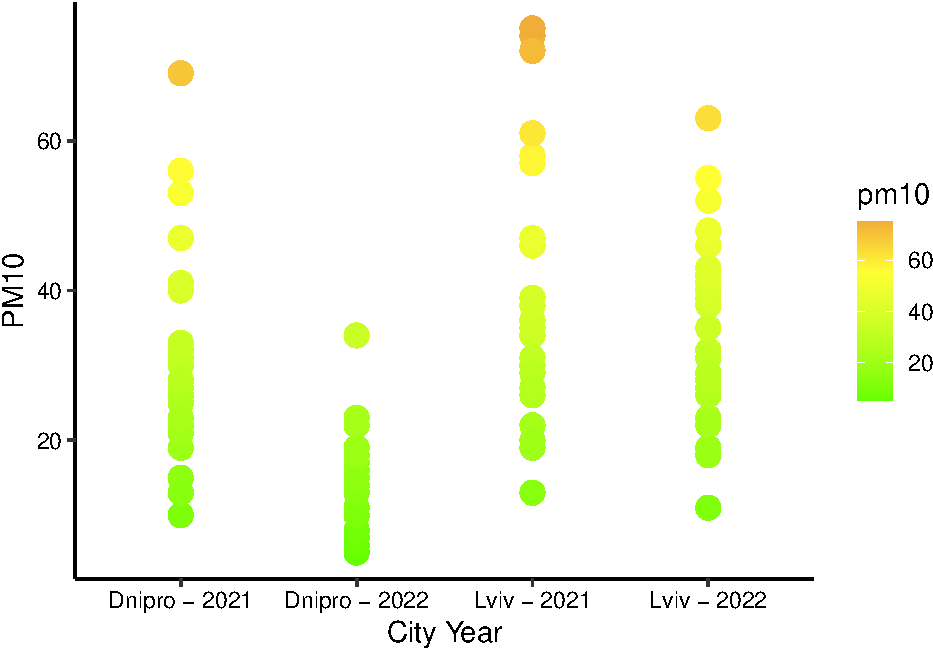
\includegraphics{Fontanie_Gordon_Weinberg_Project_files/figure-latex/plot of PM10 air pollution by city year-1.pdf}
\caption{PM10 Air Pollution Distribution}
\end{figure}

\begin{longtable}[]{@{}lrrrr@{}}
\caption{PM10 Levels by City}\tabularnewline
\toprule
City & Mean & Min & Max & Std Dev \\
\midrule
\endfirsthead
\toprule
City & Mean & Min & Max & Std Dev \\
\midrule
\endhead
Dnipro & 24.73309 & 2 & 120 & 15.82186 \\
Lviv & 30.29246 & 4 & 606 & 26.78330 \\
\bottomrule
\end{longtable}

\newpage

\hypertarget{analysis}{%
\section{Analysis}\label{analysis}}

\hypertarget{question-1-are-there-significant-differences-in-air-quality-levels-between-affected-ukrainian-cities-during-the-russian-invasion}{%
\subsection{Question 1: Are there significant differences in air quality
levels between affected Ukrainian cities during the Russian
invasion?}\label{question-1-are-there-significant-differences-in-air-quality-levels-between-affected-ukrainian-cities-during-the-russian-invasion}}

\begin{quote}
To begin our analysis, we conducted a visual analysis of PM2.5 and PM10
levels in Dnipro and Lviv for the time period of March 2022, as both
cities experienced their first missile attacks during March 2022. We
chose to use line plots including points to clearly show the values of
the PM2.5 and PM10 values. We created two different plots: ``2022 PM2.5
Levels in Dnipro and Lviv'' and ``2022 PM10 Levels in Lviv and Dnipro''.
Additionally, we conducted a linear regression analysis for each of
these charts to understand if there is a significant difference in air
quality levels in PM2.5 and PM10 between both the cities of Dnipro and
Lviv.
\end{quote}

\begin{quote}
\textbf{PM2.5 in Dnipro vs.~Lviv}\\
While plotting PM2.5 levels in Dnipro and Lviv in March 2022, we observe
significantly higher PM2.5 levels in Lviv than Dnipro consistently
throughout the month. There are just two dates where PM2.5 levels
between the cities are almost the same, March 10, 2022, and March 27,
2022. However, Lviv still shows higher PM2.5 levels than Dnipro.
According to AQI categories of PM2.5 levels, Dnipro shows PM2.5 levels
primarily in the 0 to 50 range. Therefore, Dnipro's PM2.5 AQI categories
range from ``good'' to ``moderate'' to ``poor''. Lviv shows PM2.5 levels
primarily in the 50+ values. Therefore, Lviv AQI categories range from
``poor'' to ``unhealthy''. Interestingly, Lviv shows a peak of
``unhealthy'' levels in the middle of March, while Dnipro remains
relatively stable. Overall, there is significantly more variability in
PM2.5 levels in Lviv, than Dnipro.
\end{quote}

\begin{quote}
For the statistical analysis, we ran a linear regression model of PM2.5
levels by city, to understand if there are significant differences in
PM2.5 levels between Dnipro and Lviv in March 2022. The linear
regression showed that the R-squared value of (0.5397), shows that an
estimated 54\% of variability in PM2.5 levels can be explained by the
differences in the two observed cities; Dnipro and Lviv. Additionally,
the statistical significance shows a low p-value of (p = 4.715e-11),
showing there to be a significant difference in PM2.5 levels between
Dnipro and Lviv during March 2022.
\end{quote}

\newpage

\begin{figure}
\centering
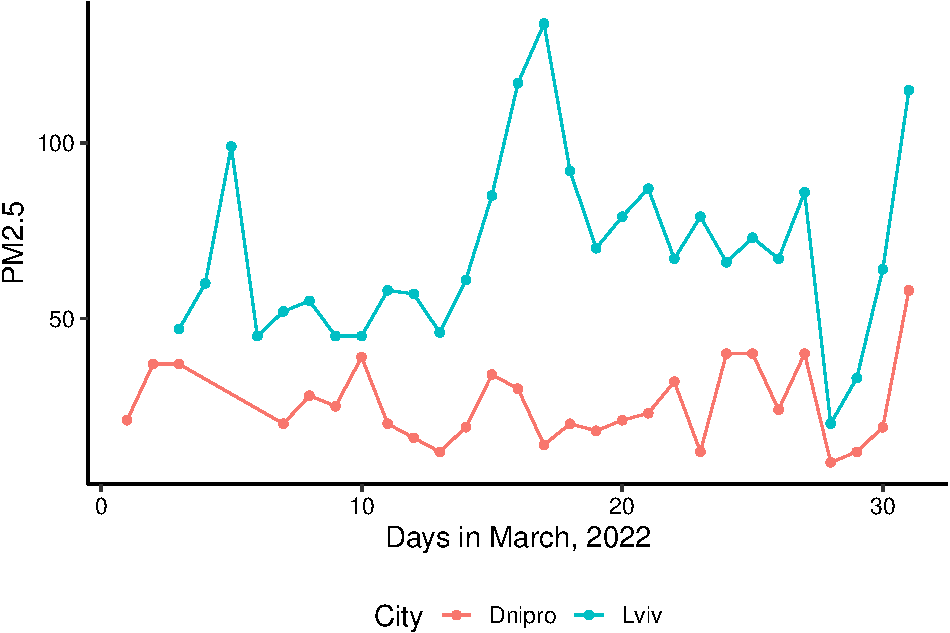
\includegraphics{Fontanie_Gordon_Weinberg_Project_files/figure-latex/Plotting Lviv vs Dnipro PM25-1.pdf}
\caption{2022 PM2.5 Levels in Dnipro and Lviv}
\end{figure}

\newpage

\begin{quote}
\textbf{PM10 in Dnipro vs.~Lviv}\\
While plotting PM10 levels in Dnipro and Lviv in March 2022, we observed
consistently higher PM10 levels in Lviv than Dnipro consistently
throughout the month. There was just one exception, when on March 9,
2022, both Dnipro and Lviv appeared to have the same PM10 level.
Following March 9, 2022, Lviv's PM10 levels skyrocketed, while Dnipro's
decreased at a relatively slower rate. According to AQI categories of
PM10 levels, Dnipro shows PM10 levels primarily in the 0 to 40 range.
Therefore, Dnipro AQI categories for PM10 are technically considered
``good''. Lviv shows PM10 levels primarily in the 20+ values. Therefore,
Lviv AQI categories range from ``good'' to ``moderate'' to ``poor''.
Similarly to our observations for PM2.5 levels as conducted above, Lviv
shows a steep increase in PM10 levels in the middle of March 2022, while
Dnipro remains relatively stable. Overall, there is significantly more
variability in PM10 levels in Lviv, than Dnipro.
\end{quote}

\begin{quote}
For the statistical analysis, we ran a linear regression model of PM10
levels by city, to understand if there are significant differences in
PM10 levels between Dnipro and Lviv in March 2022. The linear regression
showed that the R-squared value of (0.4743), shows that an estimated
47\% of variability in PM10 levels can be explained by the differences
in the two observed cities; Dnipro and Lviv. Additionally, the
statistical significance shows a low p-value of (p = 1.929e-09), showing
there to be a significant difference in PM10 levels between Dnipro and
Lviv during March 2022.
\end{quote}

\begin{figure}
\centering
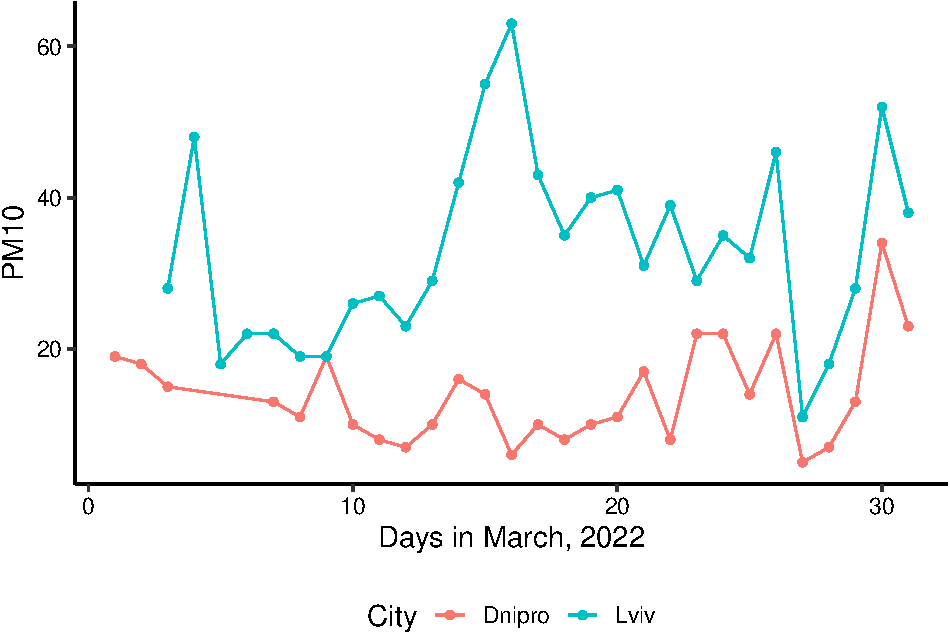
\includegraphics{Fontanie_Gordon_Weinberg_Project_files/figure-latex/Plotting Lviv and Dnipro PM10-1.pdf}
\caption{2022 PM10 Levels in Lviv and Dnipro}
\end{figure}

\newpage

\hypertarget{question-2-are-there-significant-differences-in-air-quality-levels-in-affected-ukrainian-cities-before-and-during-the-russian-attacks}{%
\subsection{Question 2: Are there significant differences in air quality
levels in affected Ukrainian cities before and during the Russian
attacks?}\label{question-2-are-there-significant-differences-in-air-quality-levels-in-affected-ukrainian-cities-before-and-during-the-russian-attacks}}

\begin{quote}
Similiar to our first research question, we conducted a visual analysis
of PM2.5 and PM10 levels within Dnipro and Lviv for years 2021 and 2022.
For each of our visualizations, we created line plots that showed the
air pollution levels within the city, comparing 2021 to 2022. As we
needed to visualize the levels of both PM2.5 and PM10, we created four
different plots - ``PM2.5 Levels in Dnipro'', ``PM2.5 Levels in Lviv'',
``PM10 Levels in Dnipro'', and ``PM10 Levels in Lviv''. Within each of
these plots, we also created annotations to indicate the specific dates
of the missile attacks within the cities to see if there were any PM2.5
or PM10 increases or decreases around those dates. Additionally, we
conducted a linear regression analysis for each of these charts to
understand if there is a significant difference in PM2.5 levels and PM10
levels within Dnipro and Lviv in March of 2021 compared to March of
2022.\\
\end{quote}

\begin{quote}
\textbf{PM2.5 in Dnipro}\\
When plotting PM2.5 levels in Dnipro in 2021 compared to 2022 (Figure
5), it is evident that overall, PM2.5 levels were higher in 2021 than
2022. It is also interesting to note that around March 11 in 2022, when
the missile attack occured, there appears to be an uptick in PM2.5
levels and then sharply decreases shortly after. Overall in both years,
there seems to be a variety of fluctuation in PM2.5 levels and they are
not consistent within each year. Additionally, within most of 2022,
PM2.5 levels stayed within ``good'' to ``moderate'' levels, with an
exception of reaching a level of ``unhealthy for sensitive groups'' at
the end of March 2022. In March 2021, however, the PM2.5 levels were
mainly in the ``unhealthy for sensitive groups'' or ``unhealthy''
category, with only a few days throughout that month in ``moderate''
levels.
\end{quote}

\begin{quote}
For the statistical analysis, we ran a linear regression model of pm2.5
levels by year within Dnipro, to understand if there are significant
differences in PM2.5 levels within the city in March 2021 compared to
March 2022. The linear regression showed the slope was negative
(-32.253), meaning that PM2.5 levels decreased in 2022 compared to 2021.
Additionally, the linear regression showed that the relationship between
PM2.5 levels and year in Dnipro is significant (p = 5.074e-10), meaning
that there is a significant difference in PM2.5 levels in Dnipro in 2022
compared to 2021.
\end{quote}

\begin{figure}
\centering
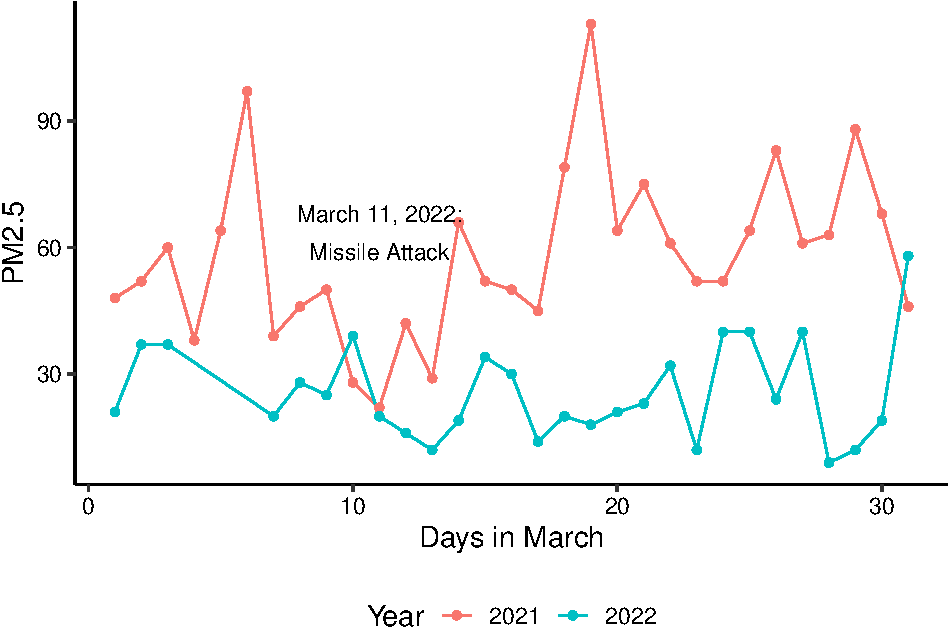
\includegraphics{Fontanie_Gordon_Weinberg_Project_files/figure-latex/Visualizing PM25 in Dnipro-1.pdf}
\caption{PM2.5 Levels in Dnipro}
\end{figure}

\newpage

\begin{quote}
\textbf{PM2.5 in Lviv}\\
When plotting PM2.5 levels in Lviv in 2021 compared to 2022 (Figure 6),
there is no clear difference in levels between years. It is interesting
to note that before the March 18 attack, PM2.5 levels were increasing,
and after the March 18, 2022 missile attack, it appears levels sharply
decreased. Overall in both years, it appears that there seems to be a
variety of fluctuation in PM2.5 in Lviv. Additionally, within both 2021
and 2022, it is very rare that levels are within the ``good'' range of
PM2.5 (\textless15.4) and are typically within ``moderate'' to
``unhealthy'' levels.
\end{quote}

\begin{quote}
For the statistical analysis, we ran a linear regression model of PM2.5
levels by year within Lviv, to understand if there are significant
differences in levels within the city in March 2021 compared to March
2022. Through the analysis, we found that the slope was negative
(-10.284), meaning that PM2.5 levels decreased in 2022 compared to 2021.
However, the linear regression showed that the negative relationship
between PM2.5 levels and year in Lviv is not significant (p=0.1639).
\end{quote}

\begin{figure}
\centering
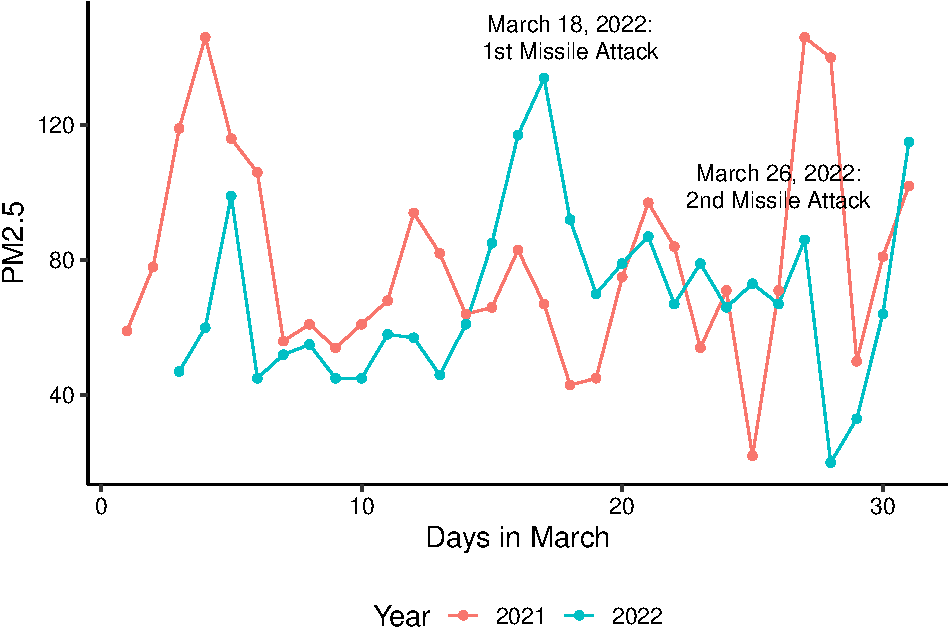
\includegraphics{Fontanie_Gordon_Weinberg_Project_files/figure-latex/visualizing PM25 in Lviv-1.pdf}
\caption{PM2.5 Levels in Lviv}
\end{figure}

\newpage

\begin{quote}
\textbf{PM10 in Dnipro}\\
When plotting PM10 levels in Dnipro in 2021 compared to 2022 (Figure 7),
it is evident that overall, PM10 levels were higher in 2021 compared to
2022. When looking at the PM10 levels around the March 11 attack in
2022, there does not appear to be a significant increase. Additionally,
in March 2022, PM10 levels seemed to stay within or below ``moderate''
levels, whereas 2021 levels ranged from ``moderate'' to ``unhealthy for
sensitive groups''.
\end{quote}

\begin{quote}
For the statistical analysis, we ran a linear regression of PM10 levels
by year within Dnipro, to understand if there are significant
differences in levels within the city in March 2021 compared to March
2022. Through the analysis, we found that the slope was negative
(-15.677), meaning that PM10 levels decreased in 2022 compared to 2021.
Additionally, the linear regression showed that these results are
statistically significant (p=4.325e-07), meaning there is a significant
difference in PM10 levels in Dnipro in 2022 compared to 2021.
\end{quote}

\begin{figure}
\centering
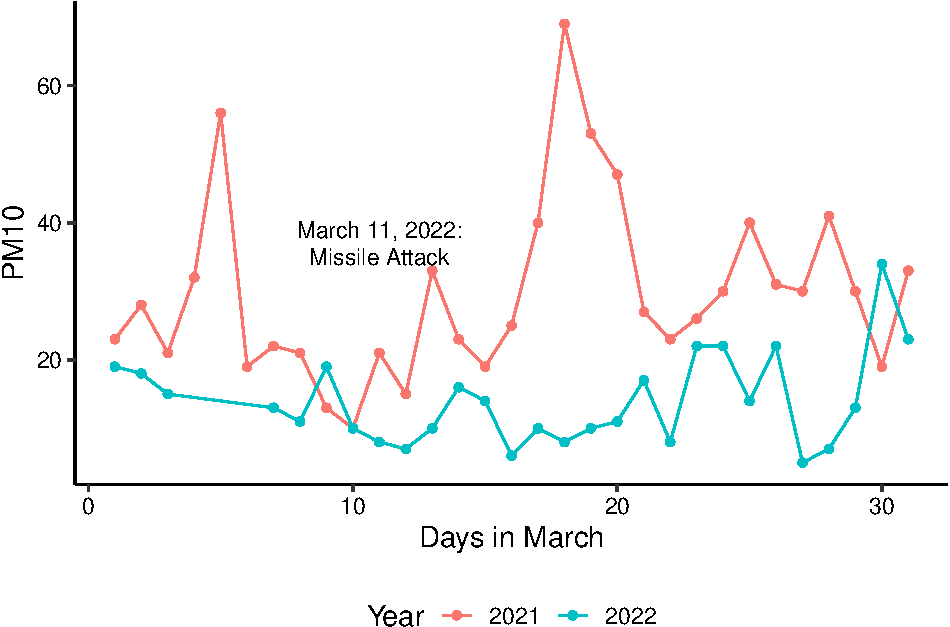
\includegraphics{Fontanie_Gordon_Weinberg_Project_files/figure-latex/visualizing PM10 in Dnipro-1.pdf}
\caption{PM10 Levels in Dnipro}
\end{figure}

\newpage

\begin{quote}
\textbf{PM10 in Lviv}\\
When plotting PM10 levels in Lviv in 2021 compared to 2022 (Figure 8),
there is no clear difference observed in PM10 levels between the years.
It is also interesting to note that there does not seem to a significant
change in PM10 levels after the March 18 attack, and PM10 levels appear
to sharply drop after the March 26 attack. Additionally, PM10 levels in
both years stay mainly within ``unhealthy for sensitive groups'' to
``good'' levels, but at some points in 2021, levels reach into the
``unhealthy'' level.
\end{quote}

\begin{quote}
For the statistical analysis, we ran a linear regression of PM10 levels
by year within Lviv, to understand if there are significant differences
in levels within the city in March 2021 compared to March 2022. Through
the analysis, we found that the slope was negative (-5.673), meaning
that PM10 levels decreased in 2022 compared to 2021 in Lviv. However,
the linear regression showed that these results are not statistically
significant (p=0.1364), meaning that there is not a significant
difference in PM10 levels in Lviv in 2022 compared to 2021.
\end{quote}

\begin{figure}
\centering
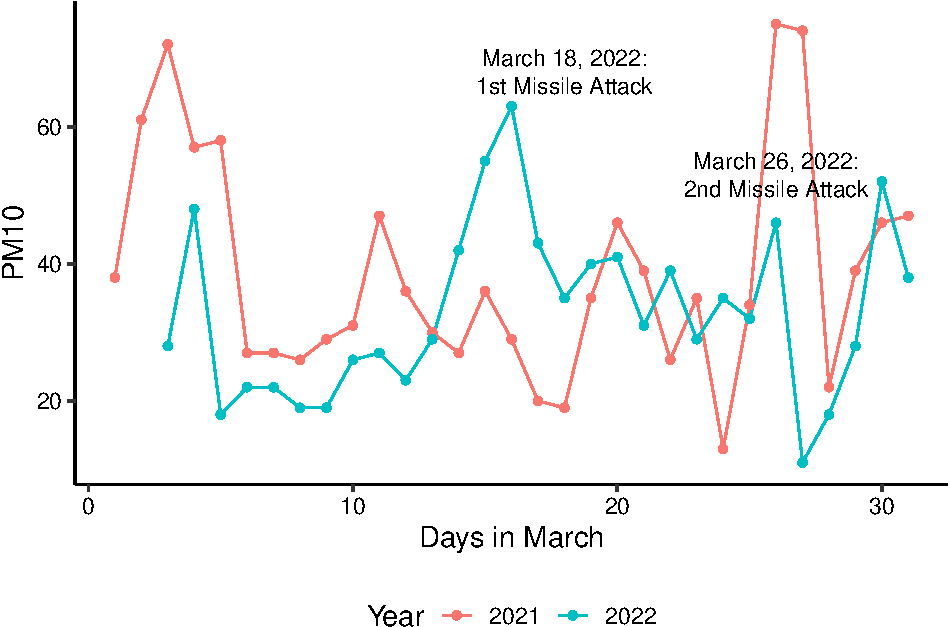
\includegraphics{Fontanie_Gordon_Weinberg_Project_files/figure-latex/visualizing PM10 in Lviv-1.pdf}
\caption{PM10 Levels in Lviv}
\end{figure}

\newpage

\hypertarget{summary-and-conclusions}{%
\section{Summary and Conclusions}\label{summary-and-conclusions}}

\hypertarget{question-1-are-there-significant-differences-in-air-quality-levels-between-affected-ukrainian-cities-during-the-russian-invasion-1}{%
\subsection{Question 1: Are there significant differences in air quality
levels between affected Ukrainian cities during the Russian
invasion?}\label{question-1-are-there-significant-differences-in-air-quality-levels-between-affected-ukrainian-cities-during-the-russian-invasion-1}}

\begin{quote}
There were significant differences in both PM2.5 and PM10 levels between
the two cities of Dnipro and Lviv during the Russian invasion in March
2022. It is important to note that while look at both levels of
particulate matter, Lviv had significantly higher PM values than Dnipro
in both PM2.5 and PM10. Lviv's PM2.5 levels, in particular, veered in
the ``unhealthy'' category, while Lviv's PM10 levels veered in the
``poor'' category. Surprisingly, Dnipro's PM10 values remained in the
``good'' to ``moderate'' range, questioning whether the bombings really
had any effect on air quality in Dnipro.
\end{quote}

\begin{quote}
These are interesting observations to discover, because while the city
of Lviv is much larger in size than Dnipro, Lviv remains a cultural
city, while Dnipro is primarily industrial. However, when looking at
both PM2.5 and PM10 levels it shows that Lviv had significantly higher
particulate matter values than Dnipro. This is an interesting
observation, and raises the question of whether the indsutrial activity
has as much of an effect on air quality as we had previously assumed.
During the Russian invasion, Ukrainains fled underground, removing all
emissions that come from daily life such as transportation. In future
studies, this is an important note to consider, and we can include more
variables such as area of city, population size, and even weather
patterns to observe how particulate matter could potentially travel
across the country.
\end{quote}

\hypertarget{question-2-are-there-significant-differences-in-air-quality-levels-in-affected-ukrainian-cities-before-and-during-the-russian-attacks-1}{%
\subsection{Question 2: Are there significant differences in air quality
levels in affected Ukrainian cities before and during the Russian
attacks?}\label{question-2-are-there-significant-differences-in-air-quality-levels-in-affected-ukrainian-cities-before-and-during-the-russian-attacks-1}}

\begin{quote}
There were significant differences in both PM2.5 and PM10 levels in
Dnipro in March of 2022 compared to March of 2021. However, there were
no significant differences in PM2.5 and PM10 levels in Lviv in March of
2022 compared to March of 2021. In Dnipro in March of 2022, the PM2.5
levels were much higher in 2021 compared to 2022, which was surprising
given the context originally discussed in which air pollution tends to
increase during times of war due to explosions and infrastructure
collapse that increase levels of hazardous dust and debris.
\end{quote}

\begin{quote}
As Dnipro typically has a high presence of industrial activity during
pre-war times, it is possible that PM2.5 and PM10 levels decreased due
to the industrial sector activities being paused during the war.
Additionally, since Lviv is more of a cultural city and does not have a
heavy industrial presence, it is likely that PM2.5 levels and PM10
levels didn't significantly change if industrial activity is a more
influential factor than presence of missile attacks. This is an
interesting idea that would be valuable to explore in future studies,
comparing multiple cities that have experienced missile attacks with
varying industrial profiles and identifying if air pollution levels
change in those cities if industrial activity is paused due to war.
\end{quote}

\begin{quote}
\textbf{Limitations}\\
It is important to note that our study was limited in the amount of data
analyzed over time. To improve the analysis, if it's possible to find
more data, we would study PM2.5 and PM10 levels from at least three
years prior. Additionally, depending on how the war continues, it would
be interested to study air pollution levels beyond March of 2022,
especially if the war worsens and there is an increasing amount of
missile attacks. Our study is also limited in the number of cities
analyzed. To improve the study, we would expand our analysis to more
cities throughout Ukraine if it is possible to find the data.
\end{quote}

\begin{quote}
Additionally, it may be valuable to explore other variables that may be
affecting air pollution levels besides war presence and missile attacks.
Specifically, population and population density may have an impact on
air pollution levels. As it was found that Lviv had much higher absolute
levels of air pollution compared to Dnipro, it would be valuable to
understand differences in population, population density, and tourism
activity (as Lviv is the cultural capital of the country) has any impact
on air pollution levels.
\end{quote}

\begin{quote}
\textbf{Conclusions}\\
From this study, we can conclude that there were differences in air
quality levels between affected cities during the Russian invasion.
However, we cannot conclude that varying levels of missile attacks is
the only factor contributing to these differences. Additionally, we can
conclude that cities may differ in air pollution levels during the
presence of war activity compared to before, however, it appears that
missile attacks may have a negative relationship with air pollution
levels. These results show that there may be other variables affecting
air pollution levels in cities (such as the presence or absence of
industrial activity) that would be valuable to analyze in future
studies.
\end{quote}

\newpage

\hypertarget{references}{%
\section{References}\label{references}}

Anna, C. (2022, March 19). Ukraine's cultural capital no longer distant
from the war. AP NEWS. Retrieved April 17, 2022, from
\url{https://apnews.com/article/russia-ukraine-kyiv-europe-religion-a3db4233f2fe7359230d4d9c56aae972}

Dathan, J. (2020, July 3). The broken land: The environmental
consequences of explosive weapon use - syrian arab republic. ReliefWeb.
Retrieved April 17, 2022, from
\url{https://reliefweb.int/report/syrian-arab-republic/broken-land-environmental-consequences-explosive-weapon-use}

EPA. (n.d.). Particulate Matter (PM) Basics. EPA. Retrieved April 17,
2022, from
\url{https://www.epa.gov/pm-pollution/particulate-matter-pm-basics}

Lister, T., Mezzofiore, G., Murphy, P., Smith-Spark, L., \& Picheta, R.
(2022, March 11). Russia widens attack on Ukraine's cities, striking
western airfields and Dnipro. CNN. Retrieved April 17, 2022, from
\url{https://www.cnn.com/2022/03/11/europe/russia-invasion-ukraine-03-11-intl/index.html}

Parrett, M. (2020, October 27). Air pollution is a problem for
manufacturing sector, according to whitepaper. New Food Magazine.
Retrieved April 17, 2022, from
\url{https://www.newfoodmagazine.com/news/122481/air-pollution/}

The World Air Quality Project. (n.d.). Air Quality Historical Data
Platform. aqicn.org. Retrieved April 17, 2022, from
\url{https://aqicn.org/data-platform/register/}

\end{document}
